%!Tex Root = ../main.tex
% ./Packete.tex
% ./Design.tex
% ./Deklarationen.tex
% ./Vorbereitung.tex
% ./Aufgabe1.tex
% ./Aufgabe2.tex
% ./Aufgabe3.tex
% ./Appendix.tex

\section{Aufgabe 4}

\setcounter{exercise}{1}

% \begin{frame}[allowframebreaks]{Aufgabe \thesection}{Implementierung eines Tristate Treibers, Transistoren}
%
% \end{frame}

    \begin{frame}[allowframebreaks]{Aufgabe \thesection}{Implementierung eines Tristate Treibers, Transistoren}
      \begin{exercisenoinc}
        % \scriptsize
        % Finde Gatter-Implementierung für $f$ und $g$ \\
        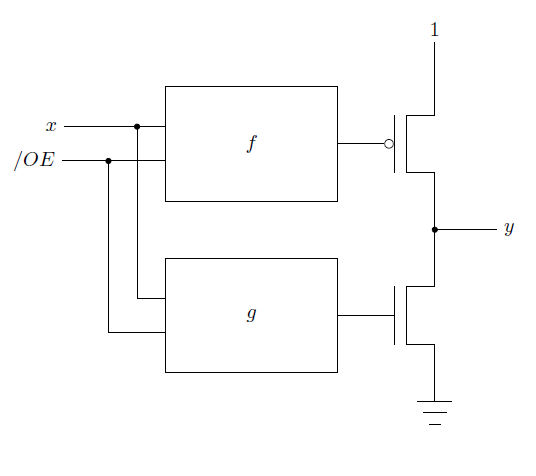
\includegraphics[height=0.5\paperheight, center]{./figures/Tristate-Treiber.png}
      \end{exercisenoinc}
      \begin{solution}
        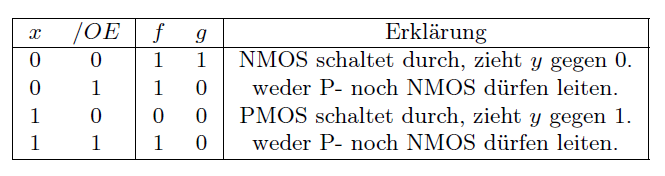
\includegraphics[width=0.8\textwidth, center]{./figures/Tristate-Treiber-Tabelle.png}\\
        \begin{columns}
          \begin{column}[t]{0.5\textwidth}
            \begin{itemize}
              \item $\begin{aligned}[t]
                  f &= \overline{x} \cdot \overline{/OE} + \overline{x} \cdot /OE + x \cdot /OE = \overline{x} + /OE\\
                    &= \overline{x \cdot \overline{ /OE}} \end{aligned}$
            \end{itemize}
          \end{column}
          \begin{column}[t]{0.5\textwidth}
            \begin{itemize}
              \item $\begin{aligned}[t]
                  g &= \overline{x} \cdot \overline{/OE} = \overline{x + /OE} \end{aligned}$
            \end{itemize}
          \end{column}
        \end{columns}
      \end{solution}
    \end{frame}

    \begin{frame}[allowframebreaks]{Aufgabe \thesection}{Implementierung eines Tristate Treibers, Transistoren}
      \begin{solutionnoinc}
        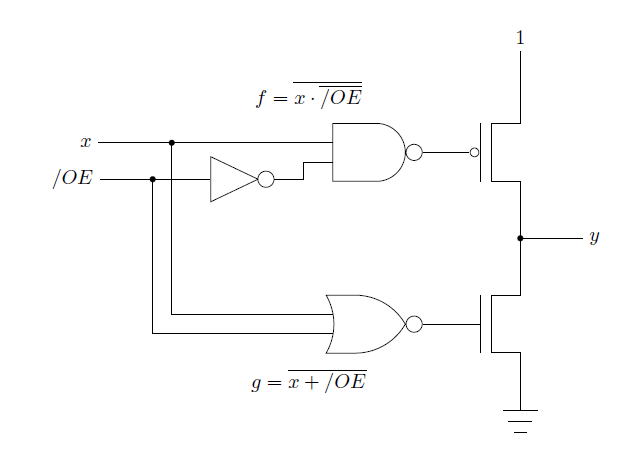
\includegraphics[height=0.5\paperheight, center]{./figures/Tristate-Treiber-Schlatkreis.png}
      \end{solutionnoinc}
      \begin{solution}
        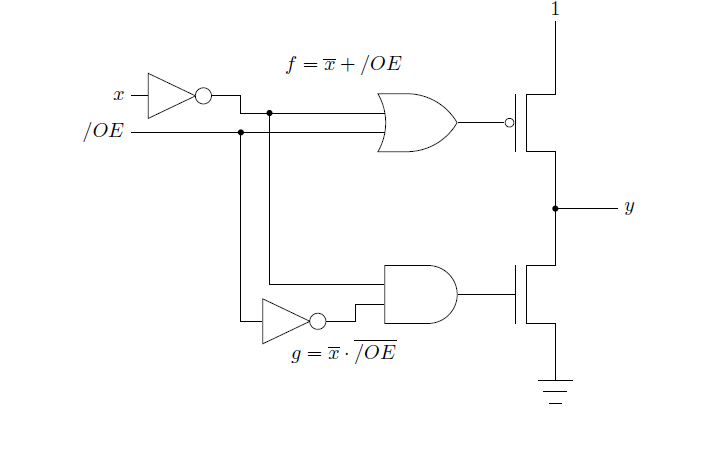
\includegraphics[height=0.5\paperheight, center]{./figures/Tristate-Treiber-Schlatkreis-Alternative.png}\\
      \end{solution}
    \end{frame}
